\documentclass[aspectratio=1610,onlymath]{beamer}
% \documentclass[aspectratio=1610,onlymath,handout]{beamer}

% Macros used by all lectures, but not necessarily by excercises

%%% General setup and dependencies:

% \usetheme[ddcfooter,nosectionnum]{tud}
\usetheme[nosectionnum,pagenum,noheader]{tud}
% \usetheme[nosectionnum,pagenum]{tud}

% Increase body font size to a sane level:
\let\origframetitle\frametitle
% \renewcommand{\frametitle}[1]{\origframetitle{#1}\normalsize}
\renewcommand{\frametitle}[1]{\origframetitle{#1}\fontsize{10pt}{13.2}\selectfont}
\setbeamerfont{itemize/enumerate subbody}{size=\small} % tud defaults to scriptsize!
\setbeamerfont{itemize/enumerate subsubbody}{size=\small}
% \setbeamerfont{normal text}{size=\small}
% \setbeamerfont{itemize body}{size=\small}

\renewcommand{\emph}[1]{\textbf{#1}}

\def\arraystretch{1.3}% Make tables even less cramped vertically

\usepackage[ngerman]{babel}
\usepackage[utf8]{inputenc}
\usepackage[T1]{fontenc}

%\usepackage{graphicx}
\usepackage[export]{adjustbox} % loads graphicx
\usepackage{import}
\usepackage{stmaryrd}
\usepackage[normalem]{ulem} % sout command
% \usepackage{times}
\usepackage{txfonts}

% \usepackage[perpage]{footmisc} % reset footnote counter on each page -- fails with beamer (footnotes gone)
\usepackage{perpage}  % reset footnote counter on each page
\MakePerPage{footnote}

\usepackage{tikz}
\usetikzlibrary{arrows,positioning}
% Inspired by http://www.texample.net/tikz/examples/hand-drawn-lines/
\usetikzlibrary{decorations.pathmorphing}
\pgfdeclaredecoration{penciline}{initial}{
    \state{initial}[width=+\pgfdecoratedinputsegmentremainingdistance,
    auto corner on length=1mm,]{
        \pgfpathcurveto%
        {% From
            \pgfqpoint{\pgfdecoratedinputsegmentremainingdistance}
                      {\pgfdecorationsegmentamplitude}
        }
        {%  Control 1
        \pgfmathrand
        \pgfpointadd{\pgfqpoint{\pgfdecoratedinputsegmentremainingdistance}{0pt}}
                    {\pgfqpoint{-\pgfdecorationsegmentaspect
                     \pgfdecoratedinputsegmentremainingdistance}%
                               {\pgfmathresult\pgfdecorationsegmentamplitude}
                    }
        }
        {%TO 
        \pgfpointadd{\pgfpointdecoratedinputsegmentlast}{\pgfpoint{1pt}{1pt}}
        }
    }
    \state{final}{}
}
\tikzset{handdrawn/.style={decorate,decoration=penciline}}
\tikzset{every shadow/.style={fill=none,shadow xshift=0pt,shadow yshift=0pt}}
% \tikzset{module/.append style={top color=\col,bottom color=\col}}

% Use to make Tikz attributes with Beamer overlays
% http://tex.stackexchange.com/a/6155
\tikzset{onslide/.code args={<#1>#2}{%
  \only<#1| handout:0>{\pgfkeysalso{#2}} 
}}
\tikzset{onslideprint/.code args={<#1>#2}{%
  \only<#1>{\pgfkeysalso{#2}} 
}}

%%% Title -- always set this first

\newcommand{\defineTitle}[3]{
	\newcommand{\lectureindex}{#1}
	\title{Formale Systeme}
	\subtitle{\href{\lectureurl}{#1. Vorlesung: #2}}
	\author{\href{http://korrekt.org/}{Markus Kr\"{o}tzsch}}
%	\author{\href{http://www.sebastian-rudolph.de}{Sebastian Rudolph} in Vertretung von \href{http://korrekt.org/}{Markus Kr\"{o}tzsch}}
	\date{#3}
	\datecity{TU Dresden}
% 	\institute{Computational Logic}
}

%%% Table of contents:

\RequirePackage{ifthen}

\newcommand{\highlight}[2]{%
	\ifthenelse{\equal{#1}{\lectureindex}}{\alert{#2}}{#2}%
}

\def\myspace{-0.7ex}
\newcommand{\printtoc}{
\begin{tabular}{r@{$\quad$}l}
\highlight{1}{1.} & \highlight{1}{Willkommen/Einleitung formale Sprachen}\\[\myspace]
\highlight{2}{2.} & \highlight{2}{Grammatiken und die Chomsky-Hierarchie}\\[\myspace]
\highlight{3}{3.} & \highlight{3}{Endliche Automaten}\\[\myspace]
\highlight{4}{4.} & \highlight{4}{Complexity of FO query answering}\\[\myspace]
\highlight{5}{5.} & \highlight{5}{Conjunctive queries}\\[\myspace]
\highlight{6}{6.} & \highlight{6}{Tree-like conjunctive queries}\\[\myspace]
\highlight{7}{7.} & \highlight{7}{Query optimisation}\\[\myspace]
\highlight{8}{8.} & \highlight{8}{Conjunctive Query Optimisation / First-Order~Expressiveness}\\[\myspace]
\highlight{9}{9.} & \highlight{9}{First-Order~Expressiveness / Introduction to Datalog}\\[\myspace]
\highlight{10}{10.} & \highlight{10}{Expressive Power and Complexity of Datalog}\\[\myspace]
\highlight{11}{11.} & \highlight{11}{Optimisation and Evaluation of Datalog}\\[\myspace]
\highlight{12}{12.} & \highlight{12}{Evaluation of Datalog (2)}\\[\myspace]
\highlight{13}{13.} & \highlight{13}{Graph Databases and Path Queries}\\[\myspace]
\highlight{14}{14.} & \highlight{14}{Outlook: database theory in practice}
\end{tabular}
}

\newcommand{\overviewslide}{%
\begin{frame}\frametitle{Overview}
\printtoc
\medskip

Siehe \href{\lectureurl}{course homepage [$\Rightarrow$ link]} for more information and materials
\end{frame}
}

%%% Colours:

\usepackage{xcolor,colortbl}
\definecolor{redhighlights}{HTML}{FFAA66}
\definecolor{lightblue}{HTML}{55AAFF}
\definecolor{lightred}{HTML}{FF5522}
\definecolor{lightpurple}{HTML}{DD77BB}
\definecolor{lightgreen}{HTML}{55FF55}
\definecolor{darkred}{HTML}{CC4411}
\definecolor{darkblue}{HTML}{176FC0}%{1133AA}
\definecolor{nightblue}{HTML}{2010A0}%{1133AA}
\definecolor{alert}{HTML}{176FC0}
\definecolor{darkgreen}{HTML}{36AB14}
\definecolor{strongyellow}{HTML}{FFE219}
\definecolor{devilscss}{HTML}{666666}

\newcommand{\redalert}[1]{\textcolor{darkred}{#1}}

%%% Style commands

\newcommand{\quoted}[1]{\texttt{"}{#1}\texttt{"}}
\newcommand{\squote}{\texttt{"}} % straight quote
\newcommand{\Sterm}[1]{\ensuremath{\mathtt{\textcolor{purple}{#1}}}}    % letters in alphabets
\newcommand{\Snterm}[1]{\textsf{\textcolor{darkblue}{#1}}} % nonterminal symbols
\newcommand{\Sntermsub}[2]{\Snterm{#1}_{\Snterm{#2}}} % nonterminal symbols
\newcommand{\Slang}[1]{\textbf{\textcolor{black}{#1}}}    % languages
\newcommand{\Slangsub}[2]{\Slang{#1}_{\Slang{#2}}}    % languages
% Code
\newcommand{\Scode}[1]{\textbf{#1}}    % reserved words in program listings, e.g., "if"
\newcommand{\Scodelit}[1]{\textcolor{purple}{#1}}    % literals in program listings, e.g., strings
\newcommand{\Scomment}[1]{\textcolor{gray}{#1}}    % comment in program listings

\newcommand{\epstrastar}{\mathrel{\mathord{\stackrel{\epsilon}{\to}}{}^*}} % transitive reflexive closure of epsilon transitions in an epslion-NFA

\newcommand{\narrowcentering}[1]{\mbox{}\hfill#1\hfill\mbox{}}

\newcommand{\defeq}{\mathrel{:=}}

\newcommand{\Smach}[1]{\ensuremath{\mathcal{#1}}}    % machines

%%% Slide layout commands:

\newcommand{\sectionSlide}[1]{
\frame{\begin{center}
\LARGE
#1
\end{center}}
}
\newcommand{\sectionSlideNoHandout}[1]{
\frame<handout:0>{\begin{center}
\LARGE
#1
\end{center}}
}

\newcommand{\mydualbox}[3]{%
 \begin{minipage}[t]{#1}
 \begin{beamerboxesrounded}[upper=block title,lower=block body,shadow=true]%
    {\centering\usebeamerfont*{block title}#2}%
    \raggedright%
    \usebeamerfont{block body}
%     \small
    #3%
  \end{beamerboxesrounded}
  \end{minipage}
}
% 
\newcommand{\myheaderbox}[2]{%
 \begin{minipage}[t]{#1}
 \begin{beamerboxesrounded}[upper=block title,lower=block title,shadow=true]%
    {\centering\usebeamerfont*{block title}\rule{0pt}{2.6ex} #2}%
  \end{beamerboxesrounded}
  \end{minipage}
}

\newcommand{\mycontentbox}[2]{%
 \begin{minipage}[t]{#1}%
 \begin{beamerboxesrounded}[upper=block body,lower=block body,shadow=true]%
    {\centering\usebeamerfont*{block body}\rule{0pt}{2.6ex}#2}%
  \end{beamerboxesrounded}
  \end{minipage}
}

\newcommand{\mylcontentbox}[2]{%
 \begin{minipage}[t]{#1}%
 \begin{beamerboxesrounded}[upper=block body,lower=block body,shadow=true]%
    {\flushleft\usebeamerfont*{block body}\rule{0pt}{2.6ex}#2}%
  \end{beamerboxesrounded}
  \end{minipage}
}

% label=180:{\rotatebox{90}{{\footnotesize\textcolor{darkgreen}{Beispiel}}}}
% \hspace{-8mm}\ghost{\raisebox{-7mm}{\rotatebox{90}{{\footnotesize\textcolor{darkgreen}{Beispiel}}}}}\hspace{8mm}
\newcommand{\examplebox}[1]{%
	\begin{tikzpicture}[decoration=penciline, decorate]
		\pgfmathsetseed{1235}
		\node (n1) [decorate,draw=darkgreen, fill=darkgreen!10,thick,align=left,text width=\linewidth, inner ysep=2mm, inner xsep=2mm] at (0,0) {#1};
% 		\node (n2) [align=left,text width=\linewidth,inner sep=0mm] at (n1.92) {{\footnotesize\raisebox{3mm}{\textcolor{darkgreen}{Beispiel}}}};
% 		\node (n2) [decorate,draw=darkgreen, fill=darkgreen!10,thick, align=left,text width=\linewidth,inner sep=2mm] at (n1.90) {{\footnotesize\raisebox{0mm}{\textcolor{darkgreen}{Beispiel}}}};
	\end{tikzpicture}%
}%

\newcommand{\codebox}[1]{%
	\begin{tikzpicture}[decoration=penciline, decorate]
		\pgfmathsetseed{1236}
		\node (n1) [decorate,draw=strongyellow, fill=strongyellow!10,thick,align=left,text width=\linewidth, inner ysep=2mm, inner xsep=2mm] at (0,0) {#1};
	\end{tikzpicture}%
}%

\newcommand{\defbox}[1]{%
	\begin{tikzpicture}[decoration=penciline, decorate]
		\pgfmathsetseed{1237}
		\node (n1) [decorate,draw=darkred, fill=darkred!10,thick,align=left,text width=\linewidth, inner ysep=2mm, inner xsep=2mm] at (0,0) {#1};
	\end{tikzpicture}%
}%

\newcommand{\theobox}[1]{%
	\begin{tikzpicture}[decoration=penciline, decorate]
		\pgfmathsetseed{1240}
		\node (n1) [decorate,draw=darkblue, fill=darkblue!10,thick,align=left,text width=\linewidth, inner ysep=2mm, inner xsep=2mm] at (0,0) {#1};
	\end{tikzpicture}%
}%

\newcommand{\anybox}[2]{%
	\begin{tikzpicture}[decoration=penciline, decorate]
		\pgfmathsetseed{1240}
		\node (n1) [decorate,draw=#1, fill=#1!10,thick,align=left,text width=\linewidth, inner ysep=2mm, inner xsep=2mm] at (0,0) {#2};
	\end{tikzpicture}%
}%


\newsavebox{\mybox}%
\newcommand{\doodlebox}[2]{%
\sbox{\mybox}{#2}%
	\begin{tikzpicture}[decoration=penciline, decorate]
		\pgfmathsetseed{1238}
		\node (n1) [decorate,draw=#1, fill=#1!10,thick,align=left,inner sep=1mm] at (0,0) {\usebox{\mybox}};
	\end{tikzpicture}%
}%

% Common notation

\usepackage{amsmath,amssymb,amsfonts}
\usepackage{xspace}

\newcommand{\lectureurl}{https://iccl.inf.tu-dresden.de/web/FS2016}

\DeclareMathAlphabet{\mathsc}{OT1}{cmr}{m}{sc} % Let's have \mathsc since the slide style has no working \textsc

% Dual of "phantom": make a text that is visible but intangible
\newcommand{\ghost}[1]{\raisebox{0pt}[0pt][0pt]{\makebox[0pt][l]{#1}}}

\newcommand{\tuple}[1]{\langle{#1}\rangle}

%%% Annotation %%%

\usepackage{color}
\newcommand{\todo}[1]{{\tiny\color{red}\textbf{TODO: #1}}}



%%% Old macros below; move when needed

\newcommand{\blank}{\text{\textvisiblespace}} % empty tape cell for TM

% table syntax
\newcommand{\dom}{\textbf{dom}}
\newcommand{\adom}{\textbf{adom}}
\newcommand{\dbconst}[1]{\texttt{"#1"}}
\newcommand{\pred}[1]{\textsf{#1}}
\newcommand{\foquery}[2]{#2[#1]}
\newcommand{\ground}[1]{\textsf{ground}(#1)}
% \newcommand{\foquery}[2]{\{#1\mid #2\}} %% Notation as used in Alice Book
% \newcommand{\foquery}[2]{\tuple{#1\mid #2}}

\newcommand{\quantor}{\mathord{\reflectbox{$\text{\sf{Q}}$}}} % the generic quantor

% logic syntax
\newcommand{\Inter}{\mathcal{I}} %used to denote an interpretation
\newcommand{\Jnter}{\mathcal{J}} %used to denote another interpretation
\newcommand{\Knter}{\mathcal{K}} %used to denote yet another interpretation
\newcommand{\Zuweisung}{\mathcal{Z}} %used to denote a variable assignment

% query languages
\newcommand{\qlang}[1]{{\sf #1}} % Font for query languages
\newcommand{\qmaps}[1]{\textbf{QM}({\sf #1})} % Set of query mappings for a query language

%%% Complexities %%%

\hyphenation{Exp-Time} % prevent "Ex-PTime" (see, e.g. Tobies'01, Glimm'07 ;-)
\hyphenation{NExp-Time} % better that than something else

% \newcommand{\complclass}[1]{{\sc #1}\xspace} % font for complexity classes
\newcommand{\complclass}[1]{\ensuremath{\mathsc{#1}}\xspace} % font for complexity classes

\newcommand{\ACzero}{\complclass{AC$_0$}}
\newcommand{\LogSpace}{\complclass{L}}
\newcommand{\NLogSpace}{\complclass{NL}}
\newcommand{\PTime}{\complclass{P}}
\newcommand{\NP}{\complclass{NP}}
\newcommand{\coNP}{\complclass{coNP}}
\newcommand{\PH}{\complclass{PH}}
\newcommand{\PSpace}{\complclass{PSpace}}
\newcommand{\NPSpace}{\complclass{NPSpace}}
\newcommand{\ExpTime}{\complclass{ExpTime}}
\newcommand{\NExpTime}{\complclass{NExpTime}}
\newcommand{\ExpSpace}{\complclass{ExpSpace}}
\newcommand{\TwoExpTime}{\complclass{2ExpTime}}
\newcommand{\NTwoExpTime}{\complclass{N2ExpTime}}
\newcommand{\ThreeExpTime}{\complclass{3ExpTime}}
\newcommand{\kExpTime}[1]{\complclass{#1ExpTime}}
\newcommand{\kExpSpace}[1]{\complclass{#1ExpSpace}}


% \usetikzlibrary{shapes}
\usetikzlibrary{shapes.geometric}

\defineTitle{19}{Nichtdeterminismus und Unentscheidbarkeit}{11. Januar 2021}

\begin{document}

\maketitle

% \begin{frame}\frametitle{}
% 
% ~\hfill
% \includegraphics[height=6.5cm]{a4}
% \hfill~
% 
% \end{frame}

% \sectionSlideNoHandout{Rückblick}
\frame{\begin{center}
\LARGE
Rückblick\bigskip

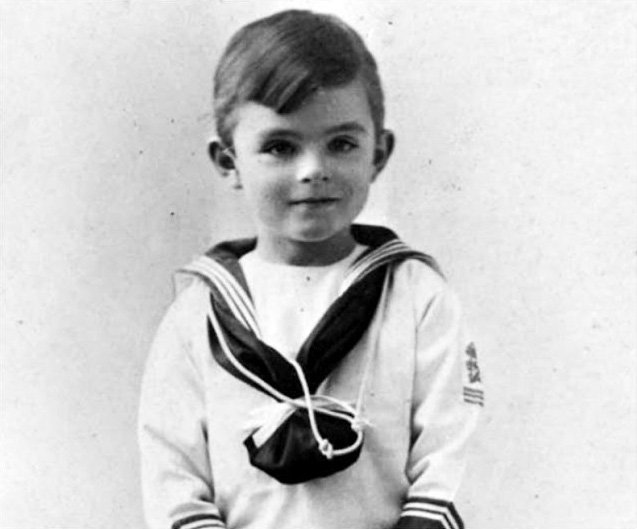
\includegraphics[height=5cm]{images/Turing-5.jpg}\\
{\tiny Alan Turing (5 Jahre alt)}
\end{center}}

\begin{frame}\frametitle{Die Turingmaschine}

\narrowcentering{%
\begin{tikzpicture}[
	scale=0.50,
	decoration=penciline, decorate
]
% \path[use as bounding box] (-3.2,0) rectangle (3.5,-5); % add "draw" to see it
% \draw[help lines] (0,0) grid (5,5);
\pgfmathsetseed{5712}
%
\node (inlabel) [rectangle,draw=none,inner sep=1pt] at (3,0.5) {\alert{Eingabe-/Speicherband}};
\draw[decorate,line width=0.3mm] (-1,0) -- (10.5,0);
\draw[decorate,line width=0.3mm] (-1,-1) -- (10.5,-1);
\foreach \x in {0,...,10} {
	\draw[decorate,line width=0.3mm] (\x-1,0) -- (\x-1,-0.9);
	\node (s\x) [circle,draw=none,inner sep=1pt] at (\x-0.5,-0.5) {\ifthenelse{\x<5}{\ifthenelse{\x<3}{\Sterm{a}}{\Sterm{b}}}{\ifthenelse{\x=5 \OR \x=7 \OR \x=8}{\Snterm{C}}{\ifthenelse{\x=9}{\Sterm{b}}{\Snterm{D}}}}};
}
\draw[decorate,line width=0.3mm] (10,0) -- (10,-0.9);
\node (dots) [circle,draw=none,inner sep=1pt] at (11.1,-0.5) {$\cdots$};

% \draw[decorate,line width=0.3mm] (5.5,0) -- (6,0) -- (6,-0.9) -- (5.5,-0.9) ;
% \draw[decorate,line width=0.3mm] (6,0) -- (6,-0.9);

\draw[fill=none,decorate,line width=0.3mm]
	(2,-3) -- (6,-3) -- (6,-7) -- (2,-7) -- cycle;
\node (falabel) [circle,draw=none,inner sep=1pt,align=left] at (4,-5) {Endliche\\Steuerung};
\draw[fill=none,decorate,line width=0.4mm,darkblue,->]
	(4,-3) -- (4,-2) -- (6.5,-2) -> (6.5,-1);
\node (headlabel) [rectangle,draw=none,inner sep=1pt,align=left] at (9.5,-2.0) {\footnotesize\alert{Lese-/Schreibkopf}\\[-0.6ex]\footnotesize\alert{(beweglich)}};

\node[rectangle,align=center,draw,line width=0.3mm,decorate, minimum width=8mm, minimum height=8mm] (state) at (8, -6) {$q$};
\draw[fill=none,decorate,line width=0.4mm,darkblue,->]
	(6,-6) -> (state.180);
\node (qlabel) [rectangle,draw=none,inner sep=1pt] at (11.5,-6) {\footnotesize\alert{Zustandsvariable}};

% \node[cloud, cloud puffs=15.7, cloud ignores aspect, minimum width=4cm, minimum height=1cm, align=center, draw,line width=0.3mm] (memory) at (11, -1) {\alert{zusätzlicher}\\\alert{Speicher}};
% 
% \draw[fill=none,decorate,line width=0.3mm] (9,0) -- (14,0);
% \draw[fill=none,decorate,line width=0.3mm] (9,-1) -- (14,-1);
% \draw[fill=none,decorate,line width=0.3mm] (9,0) -- (9,-1);
% \foreach \y in {10,...,14} {
% 	\draw[fill=none,decorate,line width=0.3mm] (\y,0) -- (\y,-0.9);
% 	\node (k\y) [circle,draw=none,inner sep=1pt] at (\y-0.5,-0.5) {\ifthenelse{\y<12}{\Snterm{A}}{\Snterm{B}}};
% }
% \draw[fill=none,decorate,line width=0.4mm,darkblue,->]
% 	(6,-3.5) -- (7.5,-3.5) -- (7.5,-0.5) -> (9,-0.5);
% \node (stacklabel) [circle,draw=none,inner sep=1pt] at (11.5,-1.5) {\alert{Warteschlange}};
\end{tikzpicture}}\bigskip

\defbox{Eine \redalert{(deterministische) Turingmaschine} (DTM) ist ein Tupel
$\Smach{M}=\tuple{Q,\Sigma,\Gamma,\delta,q_0,F}$ bestehend aus
\redalert{Zustandsmenge} $Q$, \redalert{Eingabealphabet} $\Sigma$,
\redalert{Arbeitsalphabet} $\Gamma\supseteq\Sigma\cup\{\blank\}$,
\redalert{Startzustand} $q_0\subseteq Q$, \redalert{Endzuständen} $F\subseteq Q$,
und einer partiellen \redalert{Übergangsfunktion} \\[1ex]
\narrowcentering{$\delta: Q\times\Gamma \to Q\times\Gamma\times\{L,R,N\}$}
}

\end{frame}

\begin{frame}\frametitle{Church-Turing-These}

\anybox{purple}{\emph{Church-Turing-These:} Eine Funktion ist genau dann im intuitiven Sinne berechenbar, wenn es
eine Turingmaschine gibt, die für jede mögliche Eingabe den Wert der Funktion auf das Band schreibt und anschließend hält.
}

In der Tat sind eine große Menge von Ansätzen genau gleichstark:
\begin{itemize}
\item Turingmaschinen in vielen Varianten (deterministisch/nichtdeterministisch, Einband/Mehrband,
einseitig/zweiseitig unendlich, mit/ohne wahlfreiem Zugriff, \ghost{\ldots)}
\item $\lambda$-Kalkül nach Church
\item Gödel und Herbrands allgemeine rekursive Funktionen
\item alle bekannten Programmiersprachen\footnote{Sofern wir eventuelle technische Beschränkungen der maximalen verwendbaren Speichergröße ignorieren.}
\item Typ-0-Sprachen
\item Prädikatenlogik (erster Stufe)
\end{itemize}

\end{frame}

\sectionSlide{Nichtdeterministische Turingmaschinen}

\begin{frame}\frametitle{Nichtdeterministische TMs}

\defbox{%
\redalert{Die nichtdeterministische Turingmaschine} (NTM)
\begin{enumerate}[\ldots]
\item modelliert die Übergangsfunktion als totale Funktion:\\[1ex]
\narrowcentering{$Q\times\Gamma \to 2^{Q\times\Gamma\times\{L,R,N\}}$}\\
wobei $2^{Q\times\Gamma\times\{L,R,N\}}$ die Potenzmenge von $Q\times\Gamma\times\{L,R,N\}$ ist
\item kann weiterhin mit einem einzigen Anfangszustand arbeiten
\end{enumerate}}\medskip

\redalert{Läufe} werden wie bei DTMs definiert, aber jetzt kann es pro Eingabe viele Läufe geben
\medskip

Die Eingabe wird akzeptiert, wenn mindestens ein Lauf endlich ist und in einer akzeptierenden Konfiguration endet

\end{frame}

\begin{frame}[t]\frametitle{Nichtdeterminismus $\neq$ mehr Ausdrucksstärke}

\theobox{Jede NTM ist äquivalent zu einer DTM.}\pause

\emph{Beweis:} Allgemeine Idee:
\begin{itemize}
\item Wir simulieren systematisch einen Lauf nach dem anderen
\item Die simulierende TM akzeptiert die Eingabe, wenn ein akzeptierender Lauf gefunden wird
\item Andernfalls hält sie nicht an
\end{itemize}\pause

\alert{Wie kann man systematisch alle möglichen Läufe testen?}
\begin{itemize}
\item Tiefensuche: berechne zunächst einen Lauf; falls dieser fehlschlägt, dann gehe zum letzten Entscheidungspunkt zurück und teste eine andere Möglichkeit\\\pause
$\leadsto$ Problem: nicht akzeptierende Läufe können unendlich sein\pause
%
\item Breitensuche: berechne alle Läufe bis zu einer gewissen Tiefe, für immer größere Tiefen\\
$\leadsto$ Simulation eines Laufs wird bei Maximaltiefe abgebrochen
\end{itemize}

\end{frame}

\begin{frame}[t]\frametitle{Nichtdeterminismus $\neq$ mehr Ausdrucksstärke}

\theobox{Jede NTM ist äquivalent zu einer DTM.}\pause

\emph{Beweis:} Die Simulation verwendet eine 3-Band-TM (äquivalent zu einer normalen DTM wie bereits gezeigt):
\begin{enumerate}[\color{darkblue}{Band} 1:]
\item Eingabewort (wird nie verändert)
\item Arbeitsband der simulierten NTM für aktuellen Lauf
\item Beschreibung der Übergangsentscheidungen des aktuell simulierten Laufs
\end{enumerate}\pause
Für jeden Übergang gibt es nur endlich viele Optionen, sagen wir $\ell$.\medskip\pause%

Dann kann eine Folge von Entscheidungen als Sequenz von Zahlen in $\{0,\ldots, \ell-1\}$ beschrieben werden\\
$\leadsto$ Band 3 enthält solch ein Wort über $\{0,\ldots, \ell-1\}$\medskip\pause%

Der Inhalt von Band 3 kann als \redalert{Zahl zur Basis $\ell$} gelesen werden: Um systematisch alle Optionen
zu durchsuchen, kann diese Zahl in Schritten von $1$ erhöht werden

\end{frame}

\begin{frame}[t]\frametitle{Nichtdeterminismus $\neq$ mehr Ausdrucksstärke}

\theobox{Jede NTM ist äquivalent zu einer DTM.}

\emph{Beweis:} Arbeitsweise der Simulation:\pause
\begin{enumerate}[(1)]
\item Initialisiere Band 3 mit dem Inhalt $0$\pause
\item Kopiere die Eingabe von Band 1 nach Band 2\pause
\item Simuliere einen Lauf der NTM auf Band 2. In jedem Schritt wird von Band 3 eine Zahl gelesen
und der Übergang ausgeführt, der dieser Zahl entspricht.
\begin{itemize}
\item Falls ein Übergang mit der gelesenen Zahl nicht möglich ist, gehe zu (4)
\item Falls alle Zahlen auf Band 3 gelesen sind, gehe zu (4)
\end{itemize}\pause
\item Prüfe ob die simulierte NTM in einem Endzustand angehalten hat und akzeptiere in diesem Fall, andernfalls:
\item Inkrementiere die Zahl auf Band 3 um $1$, lösche Band 2 und gehe zu Schritt (2)\qed
\end{enumerate}

\end{frame}

\begin{frame}[t]\frametitle{Komplexität und Terminierung}

\theobox{Jede NTM ist äquivalent zu einer DTM.}

\emph{Komplexität:}
Wenn die NTM einen akzeptierenden Lauf der Länge $n$ hat, dann findet ihn die DTM nach
$O(\ell^n)$ Schritten.
\medskip

$\leadsto$ \redalert{Exponentielle Komplexität}

(Es ist bis heute unbekannt, ob es eine effizientere Simulation geben könnte -- scheinbar nicht, aber der Beweis steht aus)\pause\bigskip

\emph{Terminierung:}
Wenn die NTM ein Entscheider ist (auch bei Nichtakzeptanz garantiert hält), dann ist die
simulierende DTM \ghost{\ldots}\\\pause \redalert{nicht unbedingt ein Entscheider.}
\medskip

Der Beweis kann allerdings so abgewandelt werden, dass diese Eigenschaft gilt, also:

\theobox{Jede Sprache die von einer NTM entschieden wird, kann auch von einer DTM entschieden werden.}

\end{frame}

\begin{frame}\frametitle{TM, DFA und PDA}

\redalert{Mehrband-NTMs} und ihre Äquivalenz zu 1-Band-NTMs sind analog zum deterministischen Fall.
\medskip

Damit ist leicht zu sehen:
\begin{itemize}
\item Ein DFA kann als DTM aufgefasst werden, welche die Eingabe auf dem Band nur in einer Richtung
liest und niemals beschreibt.
\item Ein PDA kann als 2-Band-NTM aufgefasst werden, die das zweite Band als Kellerspeicher verwendet
\end{itemize}

\end{frame}

\sectionSlide{Unentscheidbare Probleme}

% \frame{\begin{center}
% \LARGE
% Unentscheidbare Probleme\bigskip
% 
% \includegraphics[height=6cm]{a5.jpg}\\
% {\tiny (c) Nichtlustig, CARLSEN Verlag GmbH}
% \end{center}}

\begin{frame}\frametitle{(Un)Entscheidbarkeit}

\defbox{Eine Sprache $\Slang{L}$ ist \redalert{entscheidbar} (=\redalert{berechenbar}=\redalert{rekursiv}), wenn es eine TM $\Smach{M}$ gibt, die ihr Wortproblem entscheidet, d.h. $\Smach{M}$ ist Entscheider und $\Slang{L}=\Slang{L}(\Smach{M})$.
Andernfalls heißt $\Slang{L}$ \redalert{unentscheidbar}.\\[1ex]
$\Slang{L}$ ist \redalert{semi-entscheidbar} (=\redalert{Turing-erkennbar}=\redalert{rekursiv aufzählbar}), wenn
es eine TM $\Smach{M}$ gibt mit $\Slang{L}=\Slang{L}(\Smach{M})$, auch wenn $\Smach{M}$ kein Entscheider ist.}\medskip\pause

% $\leadsto$ "`semi-entscheidbar"' = "`Turing-erkennbar"' = "`rekursiv aufzählbar"'\\
% $\leadsto$ "`entscheidbar"' = "`berechenbar"' = "`rekursiv"'\medskip

\examplebox{Beispiel: Wir haben bereits erwähnt, dass die Äquivalenz zweier kontextfreier Grammatiken (CFGs) unentscheidbar ist.
Sei $\textsf{enc}(G)$ eine (beliebige) binäre Kodierung der Regeln einer Grammatik $G$. Das erwähnte Resultat bedeutet formal, dass die Sprache\\[1ex]
% 
\narrowcentering{$\{\textsf{enc}(G_1)\Sterm{\#}\textsf{enc}(G_2)\mid \Slang{L}(G_1)=\Slang{L}(G_2)\text{ oder }G_1\text{ bzw. }G_2\text{ keine CFG}\}$}\\[1ex]
% 
über dem Alphabet $\{\Sterm{0},\Sterm{1},\Sterm{\#}\}$ unentscheidbar ist.
}

% Aber wie kann man das zeigen?

\end{frame}

\begin{frame}\frametitle{Ein konkretes unentscheidbares Problem}

Wir wissen bereits:
\theobox{Satz: Es gibt abzählbar viele Turingmaschinen (Computerprogramme, Algorithmen) aber überabzählbar viele
Sprachen. Also sind die meisten Sprachen unentscheidbar.}

Das liefert allerdings kein konkretes Beispiel für so eine Sprache.
\bigskip\pause

Wir benötigen ein "`erstes"' unentscheidbares Problem. Das folgende ist klassisch:

\defbox{Das \redalert{Halteproblem} besteht in der folgenden Frage:\\
Gegeben eine TM $\Smach{M}$ und ein Wort $w$, wird $\Smach{M}$ für die Eingabe $w$ jemals anhalten?}

Wir wollen zeigen, dass dieses Problem unentscheidbar ist.

\end{frame}

\begin{frame}\frametitle{Turingmaschinen kodieren}

Will man das Halteproblem als Wortproblem ausdrücken, dann muss man eine Kodierung für
TMs als Wörter festlegen.
\medskip

Jede vernünftige Kodierung einer TM $\Smach{M}=\tuple{Q,\Sigma,\Gamma,\delta,q_0,F}$ ist nutzbar, zum Beispiel die folgende:

\anybox{gray}{%
\footnotesize\vspace{-2ex}%
\begin{itemize}
\item Wir verwenden das Alphabet $\{\Sterm{0},\Sterm{1},\Sterm{\#}\}$
\item Zustände werden in beliebiger Reihenfolge nummeriert (mit Startzustand $q_0$) und binär kodiert:\\
	$Q=\{q_0,\ldots,q_n\}$ $\leadsto$ $\textsf{enc}(Q)=\textsf{bin}(0)\Sterm{\#}\cdots\Sterm{\#}\textsf{bin}(n)$
\item Wir kodieren auch $\Gamma$ und die Bewegungsrichtungen $\{R,L,N\}$ binär
\item Ein Übergang $\delta(q_i,\sigma_n)=\tuple{q_j,\sigma_m,D}$ wird als 5-Tupel kodiert:\\
	 $\textsf{enc}(q_i,\sigma_n)=\textsf{bin}(i)\Sterm{\#}\textsf{bin}(n)\Sterm{\#}\textsf{bin}(j)\Sterm{\#}\textsf{bin}(m)\Sterm{\#}\textsf{bin}(D)$
\item Die Übergangsfunktion wird kodiert als Liste aller dieser Tupel, getrennt mit $\Sterm{\#}$:
	$\textsf{enc}(\delta)=\big(\textsf{enc}(q_i,\sigma_n)\Sterm{\#}\big)_{q_i\in Q, \sigma_i\in\Gamma}$
\item Insgesamt setzten wir $\textsf{enc}(\Smach{M})=\textsf{enc}(Q)\Sterm{\#}\Sterm{\#}\textsf{enc}(\Sigma)\Sterm{\#}\Sterm{\#}\textsf{enc}(\Gamma)\Sterm{\#}\Sterm{\#}\textsf{enc}(\delta)\Sterm{\#}\Sterm{\#}\textsf{enc}(F)$
\end{itemize}}

\end{frame}

\begin{frame}\frametitle{Das Halteproblem, formal}

Analog kann man auch Wörter über beliebigen $\Sigma$ binär kodieren.
\medskip

Damit kann man formal auch sagen:

\defbox{Das \redalert{Halteproblem} ist das Wortproblem für die Sprache\\[1ex]
\narrowcentering{
$\{\textsf{enc}(\Smach{M})\Sterm{\#}\Sterm{\#}\textsf{enc}(w)\mid \text{$\Smach{M}$ hält bei Eingabe $w$}\}$.
}}\pause

\emph{Anmerkung:} Wörter aus $\{\Sterm{0},\Sterm{1},\Sterm{\#}\}^*$, die nicht die Form
$\textsf{enc}(\Smach{M})\Sterm{\#}\Sterm{\#}\textsf{enc}(w)$ haben (z.B. weil die Kodierungen fehlerhaft sind), werden
laut dieser Definition abgelehnt.\medskip

$\leadsto$ typisch für Entscheidungsprobleme:\\
\hspace{1cm}\alert{Akzeptanz:} Antwort auf Frage ist "`ja"'\\
\hspace{1cm}\alert{Ablehnung:} Antwort auf Frage ist "`nein"' \redalert{oder}\\
\hspace{2.74cm}die Eingabe kodiert gar keine Frage

\end{frame}

\begin{frame}[t]\frametitle{Unentscheidbarkeit des Halteproblems}

\theobox{Das Halteproblem ist unentscheidbar.}

\emph{Beweis:} Mittels Widerspruch: Angenommen, es gäbe eine DTM \ghost{$\Smach{H}$,}\\
die das
Halteproblem entscheidet, d.h. $\Smach{H}$ hält immer und akzeptiert Eingaben $\textsf{enc}(\Smach{M})\Sterm{\#}\Sterm{\#}\textsf{enc}(w)$ genau dann wenn $\Smach{M}$ auf $w$ hält.
\medskip\pause

Wir verwenden $\Smach{H}$ als Subroutine einer neuen DTM $\Smach{D}$, die sich wie folgt verhält:\pause
\begin{enumerate}[(1)]
\item $\Smach{D}$ schreibt eine Eingabe $w\in\{\Sterm{0},\Sterm{1},\Sterm{\#}\}$ zunächst in die Form
	$w\Sterm{\#}\Sterm{\#}\textsf{enc}(w)$ um.\pause
\item Dann führt $\Smach{D}$ die TM $\Smach{H}$ auf dieser Eingabe aus.\pause
\item Wenn $\Smach{H}$ die Eingabe \redalert{nicht} akzeptiert, dann hält $\Smach{D}$ und akzeptiert.\pause
\item Andernfalls, wenn $\Smach{H}$ die Eingabe akzeptiert, dann geht $\Smach{D}$ in eine Endlosschleife und hält nicht.\pause
\end{enumerate}
\emph{Idee:} $\Smach{D}$ hält (und akzeptiert) eine TM-Kodierung $\textsf{enc}(\Smach{M})$ genau dann, wenn
$\Smach{M}$ auf der Eingabe $\textsf{enc}(\Smach{M})$ \redalert{nicht} hält.

\end{frame}

\begin{frame}[t]\frametitle{Unentscheidbarkeit des Halteproblems (2)}

\theobox{Das Halteproblem ist unentscheidbar.}

\emph{Beweis:} $\Smach{D}$ hält (und akzeptiert) eine TM-Kodierung $\textsf{enc}(\Smach{M})$ genau dann, wenn
$\Smach{M}$ auf der Eingabe $\textsf{enc}(\Smach{M})$ \redalert{nicht} hält.\pause
\medskip

\redalert{Was tut $\Smach{D}$ für die Eingabe $\textsf{enc}(\Smach{D})?$}\pause
\begin{itemize}
\item Falls $\Smach{D}$ auf Eingabe $\textsf{enc}(\Smach{D})$ hält, dann akzeptiert $\Smach{H}$
die Eingabe $\textsf{enc}(\Smach{D})\Sterm{\#}\Sterm{\#}\textsf{enc}(\textsf{enc}(\Smach{D}))$,
doch dann (laut Definition) hält $\Smach{D}$ nicht!\pause
\item Falls $\Smach{D}$ auf Eingabe $\textsf{enc}(\Smach{D})$ nicht hält, dann akzeptiert $\Smach{H}$
die Eingabe $\textsf{enc}(\Smach{D})\Sterm{\#}\Sterm{\#}\textsf{enc}(\textsf{enc}(\Smach{D}))$ nicht,
doch dann (laut Definition) hält $\Smach{D}$!
\end{itemize}
Widerspruch.\qed

\end{frame}

\begin{frame}\frametitle{Die Universelle Turingmaschine}

% Allerdings ist das Halteproblem semi-entscheidbar:\medskip

\theobox{Satz: Es gibt eine Turingmaschine $\Smach{U}$, die für Eingaben der Form $\textsf{enc}(\Smach{M})\Sterm{\#}\Sterm{\#}\textsf{enc}(w)$ das Verhalten von $\Smach{M}$ auf $w$ simuliert:
\begin{itemize}
\item Falls $\Smach{M}$ auf $w$ hält, dann hält $\Smach{U}$ auf $\textsf{enc}(\Smach{M})\Sterm{\#}\Sterm{\#}\textsf{enc}(w)$ mit dem gleichen Ergebnis
\item Falls $\Smach{M}$ auf $w$ nicht hält, dann hält $\Smach{U}$ auf $\textsf{enc}(\Smach{M})\Sterm{\#}\Sterm{\#}\textsf{enc}(w)$ ebenfalls nicht
\end{itemize}}

\defbox{Eine TM $\Smach{U}$ wie im Satz heißt \redalert{Universelle Turingmaschine (UTM)}.}

Es ist etwas aufwändig aber nicht sehr kompliziert eine UTM zu beschreiben
\medskip

\emph{Intuitiv gleichwertig:} Programmieren eines TM-Simulators in einer beliebigen Programmiersprache

\end{frame}

\begin{frame}\frametitle{Semi-Entscheidbarkeit des Halteproblems}

\theobox{Satz: Das Halteproblem ist semi-entscheidbar.}

\emph{Beweisskizze:} Die gesuchte TM startet eine universelle TM auf der Eingabe 
und akzeptiert, wenn diese UTM hält (egal mit welchem Ergebnis).\qed

\bigskip
\emph{Anmerkung:} Falls die Antwort auf das Halteproblem "`nein"' ist, dann wird auch diese
TM nicht halten.

\end{frame}

\begin{frame}\frametitle{Nicht Turing-erkennbare Probleme}

Das Komplement des Halteproblems ("`Wird die gegebene TM nicht anhalten?"') liefert 
ein Beispiel für ein Problem, welches unentscheidbar und nicht semi-entscheidbar ist:
\medskip

\theobox{Satz: Das Komplement des Halteproblems ist nicht Turing-erkennbar.}

\emph{Beweisskizze:} Angenommen das Problem wäre Turing-erkennbar.
Dann könnten wir
das Halteproblem entscheiden, indem wir die Semi-Entscheidungsalgorithmen für Halteproblem
und sein Komplement parallel abarbeiten. Einer der beiden Algorithmen muss halten und liefert
dann das gesuchte Ergebnis. Widerspruch.\qed

\end{frame}

\begin{frame}\frametitle{Turing-Mächtigkeit}

\defbox{%
Ein Formalismus ist \redalert{Turing-mächtig}, wenn er das Ein-/Ausgabe-Verhalten jeder Turing-Maschine simulieren kann\\
(äquivalent: wenn er eine UTM kodieren kann).}\bigskip

\emph{Vorteil:} Turing-Mächtigkeit garantiert ein Maximum an Ausdrucksstärke\\
$\leadsto$ gewünscht besonders bei Programmiersprachen
\bigskip

\emph{Nachteil:} Turing-Mächtigkeit bedeutet, dass alle interessanten Fragen in Bezug auf die berechnete Funktion unentscheidbar sind (z.B. Äquivalenz zweier Darstellungen) \\
$\leadsto$ zumeist unerwünscht, wenn nicht programmiert wird

\end{frame}

\begin{frame}\frametitle{Versehentlich Turing-mächtig (1)}

Immer wieder stellen sich bestimmte Technologien und formale Systeme unerwartet als
Turing-mächtig heraus.\pause
\vspace{3mm}

\anybox{purple}{
{\large \alert{C++ Templates}}
\bigskip

Ein Mechanismus zur generischen Programmierung in C++, bei dem zur Compilezeit (beliebig viele) Code-Templates instantiiert werden. Damit lassen sich TMs simulieren. Daher ist das Halteproblem für C++-Compiler unentscheidbar.
Sogar die Frage, ob eine gegebene Textdatei ein gültiges C++-Programm ist, ist unentscheidbar.
Praktisch wurde demonstriert, wie der Compiler Primzahlen berechnen und als Compilerfehler ausgeben kann.
}

\end{frame}

\begin{frame}\frametitle{Versehentlich Turing-mächtig (2)}

Immer wieder stellen sich bestimmte Technologien und formale Systeme unerwartet als
Turing-mächtig heraus.
\vspace{3mm}

\anybox{purple}{
{\large \alert{Sendmail:}}
\bigskip

SMTP-Server, welcher die automatische Umschreibung von Emails mit Regeln unterstützt.
Die Zeichenketten können in diesem Zusammenhang fast direkt als Speicherband verwendet werden (ähnliche Effekte gibt es bei anderen String-Umschreibungs-Systemen, wie Apache Rewrite Rules, wenn diese nicht in ihrer Rekursionstiefe beschränkt werden).
}

\end{frame}

\begin{frame}\frametitle{Versehentlich Turing-mächtig (3)}

Immer wieder stellen sich bestimmte Technologien und formale Systeme unerwartet als
Turing-mächtig heraus.
\vspace{3mm}

\anybox{purple}{
{\large \alert{X86 Memory Management Unit:}}
\bigskip

Hardwarekomponente einer verbreiteten Computerarchitektur.
Die Verarbeitung von Seitenfehlern (page faults) kann genutzt werden, um eine Turing-vollständige Berechnung
in Gang zu setzten, ohne die CPU zu verwenden. Demonstriert wurde eine Implementierung von Conway's Game of Life.
}

\end{frame}

\begin{frame}\frametitle{Versehentlich Turing-mächtig (4)}

Immer wieder stellen sich bestimmte Technologien und formale Systeme unerwartet als
Turing-mächtig heraus.
\vspace{3mm}

\anybox{purple}{
{\large \alert{SQL:}}
\bigskip

Verbreitete Anfragesprache für relationale Datenbanken. Mit Hilfe von rekursiven Hilfstabellen
(Common Table Expressions/\texttt{WITH RECURSIVE}) kann eine einzelne Abfrage Turingmaschinen simulieren.
}

\end{frame}

\begin{frame}\frametitle{Versehentlich Turing-mächtig (5)}

Immer wieder stellen sich bestimmte Technologien und formale Systeme unerwartet als
Turing-mächtig heraus.
\vspace{3mm}

\anybox{purple}{
{\large \alert{Magic: The Gathering:}}
\bigskip

Populäres Tauschkartenspiel. Es ist möglich, einen
Spielverlauf zu konstruieren, bei dem Spieler fast keine Entscheidungen treffen müssen und die komplexen 
Spielregeln automatisch zur Entwicklung einer TM-Simulation führen. Dabei wird ein Stapelspeicher als Reihe
von Zombies mit linear ansteigenden Lebenspunkten repräsentiert.
}

\end{frame}

\begin{frame}\frametitle{Versehentlich Turing-mächtig (6)}

Immer wieder stellen sich bestimmte Technologien und formale Systeme unerwartet als
Turing-mächtig heraus.
\vspace{3mm}

\anybox{purple}{
{\large \alert{Java Generics:}}
\bigskip

Mechanismus zur generischen Programmierung in Java. Sollte die Turing-Vollständigkeit
von C++-Templates vermeiden. Offenbar ist das nicht gelungen. Erstmals publiziert Mai 2016.
}


\end{frame}

\begin{frame}\frametitle{Versehentlich Turing-mächtig (7)}

Immer wieder stellen sich bestimmte Technologien und formale Systeme unerwartet als
Turing-mächtig heraus.
\vspace{3mm}

\anybox{purple}{
{\large \alert{Microsoft Powerpoint:}}
\bigskip
Programm zum Erstellen von Präsentationen. Simulationen von Turing-Maschinen
auf beliebigem aber begrenztem Speicher können allein durch Animationen, Links
und AutoShapes (ohne VB Makros etc.) realisiert werden. Praktisch wurde lediglich demonstriert, wie man Palindrome gerader Länge erkennen kann. Veröffentlicht April 2017.\\
\href{https://youtu.be/uNjxe8ShM-8}{[Video]} \href{https://www.andrew.cmu.edu/user/twildenh/PowerPointTM/Paper.pdf}{[Paper]}
}

(Weitere Beispiele siehe \url{http://beza1e1.tuxen.de/articles/accidentally_turing_complete.html}.)

\end{frame}

\begin{frame}\frametitle{Zusammenfassung und Ausblick}

\redalert{Nichtdeterministische Turingmaschinen} (NTMs) haben die gleiche Ausdruckstärke wie deterministische
\bigskip

Das \redalert{Halteproblem} ist unentscheidbar und sein Komplement ist nicht einmal semi-entscheidbar.
\bigskip

Es gibt sehr viele \redalert{Turing-mächtige} Systeme. Das ist nicht immer erwünscht.
\bigskip

\anybox{yellow}{
Offene Fragen:
\begin{itemize}
\item Wie ergibt sich die Korrespondenz von TMs und Typ-0-Sprachen?
\item Wenn alle Modelle Typ 0 liefern, was ist dann mit Typ 1?
\item Unterscheiden sich Typ 0 und Typ 1 überhaupt?
\end{itemize}
}

\end{frame}

% \begin{frame}\frametitle{Frohe Weihnachten!}
% 
% 
% \narrowcentering{%
% \scalebox{0.75}{
% \begin{tikzpicture}[
% 	scale=1.80,
% 	decoration=penciline, decorate,
% 	node distance = 7mm and 9mm
% ]
% \path[use as bounding box] (-3.5,-1.1) rectangle (3.5,-5); % add "draw" to see it
% \pgfmathsetseed{6571}
% 
% 
% % \draw[help lines] (0,0) grid (5,5);
% \node (s) [star,star points=5, star point ratio=2.25,draw=red,fill=strongyellow,inner sep=1pt] at (0,-0.8) {\Snterm{S}};
% % 
% \only<2->{
% \node (label) [rectangle,draw=none,color=purple,inner sep=3pt] at (2,-1.5) {\large "`dorr kleene Stern"'};
% \path[fill=none,draw=purple,line width=0.5mm,bend right=45] (label.130) edge[->] (0.4,-0.65);
% }
% % 
% %
% \node (a12) [circle,draw=none,inner sep=0pt] at (0,-1.5) {\Snterm{A}};
% % 
% \draw[fill=none,decorate,line width=0.3mm]
% (s.270) -- (-1.3,-3.5) -- (1.3,-3.5) -- cycle;
% %
% \draw[decorate,dashed,line width=0.2mm]
% (s.270) -- (a12.90);
% %
% \draw[fill=darkgreen!30,decorate,line width=0.3mm]
% (a12.270) -- (-1.0,-3.50) -- (1.0,-3.52) -- cycle;
% %
% \node (a11) [circle,draw=none,inner sep=0pt] at (0,-2.5) {\Snterm{A}};
% %
% \draw[decorate,dashed,line width=0.2mm]
% (a12.270) -- (a11.90);
% %
% \draw[fill=darkgreen!30,decorate,line width=0.3mm]
% (a11.270) -- (-1.0,-4.50) -- (1.0,-4.52) -- cycle;
% %
% \node (a1) [circle,draw=none,inner sep=0pt] at (0,-3.5) {\Snterm{A}};
% %
% \draw[decorate,dashed,line width=0.2mm]
% (a11.270) -- (a1.90);
% %
% \draw[fill=darkgreen!30,decorate,line width=0.3mm]
% (a1.270) -- (-1.0,-5.50) -- (1.0,-5.52) -- cycle;
% %
% \node (a2) [circle,draw=none,inner sep=0pt] at (0,-4.5) {\Snterm{A}};
% %
% \draw[decorate,dashed,line width=0.2mm]
% (a1.270) -- (a2.90);
% %
% \draw[fill=darkred!30,decorate,line width=0.3mm]
% (a2.270) -- (-0.5,-5.51) -- (0.5,-5.54) -- cycle;
% %
% \draw [thick, devilscss,decorate,decoration={brace,amplitude=3pt,mirror},xshift=0.4pt,yshift=-1mm](-1.3,-3.5) -- (-1.0,-3.5) node[black,midway,yshift=-0.25cm] {$u$};
% \draw [thick, devilscss,decorate,decoration={brace,amplitude=3pt,mirror},xshift=0.4pt,yshift=-1.3mm](-1.0,-3.5) -- (-0.5,-3.5) node[black,midway,yshift=-0.28cm] {$v$};
% \draw [thick, devilscss,decorate,decoration={brace,amplitude=3pt,mirror},xshift=0.4pt,yshift=-1mm](0.5,-3.5) -- (1,-3.5) node[black,midway,yshift=-0.25cm] {$x$};
% \draw [thick, devilscss,decorate,decoration={brace,amplitude=3pt,mirror},xshift=0.4pt,yshift=-0.7mm](1.0,-3.5) -- (1.3,-3.5) node[black,midway,yshift=-0.26cm] {$y$};
% 
% \draw [thick, devilscss,decorate,decoration={brace,amplitude=3pt,mirror},xshift=0.4pt,yshift=-1.3mm](-1.0,-4.5) -- (-0.5,-4.5) node[black,midway,yshift=-0.28cm] {$v$};
% \draw [thick, devilscss,decorate,decoration={brace,amplitude=3pt,mirror},xshift=0.4pt,yshift=-1mm](0.5,-4.5) -- (1,-4.5) node[black,midway,yshift=-0.25cm] {$x$};
% 
% \draw [thick, devilscss,decorate,decoration={brace,amplitude=3pt,mirror},xshift=0.4pt,yshift=-1.3mm](-1.0,-5.5) -- (-0.5,-5.5) node[black,midway,yshift=-0.28cm] {$v$};
% \draw [thick, devilscss,decorate,decoration={brace,amplitude=3pt,mirror},xshift=0.4pt,yshift=-1mm](0.5,-5.5) -- (1,-5.5) node[black,midway,yshift=-0.25cm] {$x$};
% \draw [thick, devilscss,decorate,decoration={brace,amplitude=3pt,mirror},xshift=0.4pt,yshift=-1.5mm](-0.5,-5.5) -- (0.5,-5.5) node[black,midway,yshift=-0.3cm] {$w$};
% %
% % \draw [thick, alert,decorate,decoration={brace,amplitude=10pt,mirror},xshift=0.4pt,yshift=-0.4cm](-1.5,-3.5) -- (1.5,-3.5) node[black,midway,yshift=-0.55cm] {\alert{abgeleitetes Wort}};
% \end{tikzpicture}}}
% 
% \end{frame}


\end{document}
